\documentclass[12pt]{article}
\usepackage[spanish]{babel}
\usepackage{fancyhdr}
\usepackage{multicol}
\usepackage{tasks}
\usepackage[margin=2.5cm]{geometry}

\usepackage{graphicx}
\usepackage{float}

\setlength{\parskip}{1.5mm}
\setlength{\parindent}{0pt}
\setlength{\headsep}{3mm}

\usepackage{amsthm}
\usepackage{amsmath}
\usepackage{amssymb}

\allowdisplaybreaks
\spanishdecimal{.}
\usepackage{ifthen}
\usepackage{tcolorbox}
\usepackage{varwidth}

\tcbuselibrary{theorems}
\tcbuselibrary{breakable}
\tcbuselibrary{skins}
\theoremstyle{definition}

%With section
\newtheorem{lemma}{Lema}[section]
\newtheorem{example}{Ejemplo}[section]
\newtheorem{theorem}{Teorema}[section]
\newtheorem{problem}{Problema}[section]
\newtheorem{property}{Propiedad}[section]
\newtheorem{exercise}{Ejercicio}[section]
\newtheorem{corollary}{Corolario}[section]
\newtheorem{definition}{Definición}[section]

%Without numeration
\newtheorem*{note}{Nota}
\newtheorem*{hint}{Pista}

\newenvironment{solution}[1][]
{
    \begin{proof}[\textnormal{\textbf{Solución\ifthenelse{\equal{#1}{}}{}{ #1}}}]
    }{
    \end{proof}
}


\newtcbtheorem[use counter*= theorem, number within=section]{theorem.box}{Teorema}
{
    enhanced
    ,colback = gray!10!white
    ,frame hidden
    ,boxrule = 0sp
    ,borderline west = {2.5pt}{0pt}{black}
    ,sharp corners
    ,attach title to upper
    ,coltitle = black
    ,fonttitle = \bfseries
    ,description font = \mdseries
    ,separator sign none,
    ,terminator sign={.\hspace{2mm}}
    ,description delimiters parenthesis,
    right=1mm,
    top=0mm,
    left=1.5mm,
    bottom=0mm,
    breakable = true
}
{t}



\newtcbtheorem[number within=section]{definition.tcb}{Definición}
{
    enhanced,
    frame empty,
    interior empty,
    coltitle = black,
    colbacktitle = gray!15!white,
    fonttitle = \bfseries,
    extras broken = {frame empty, interior empty},
    borderline = {0.3mm}{0mm}{black},
    breakable = true,
    top = 4mm,
    before skip = 3.5mm,
    attach boxed title to top left = {yshift = -3mm, xshift = 3mm},
    boxed title style = {boxrule = 0mm, borderline = {0.1mm}{0mm}{black}},
    varwidth boxed title,
    separator sign none, description delimiters parenthesis,
    description font=\bfseries,
    terminator sign={.\hspace{1mm}}
}
{d}


\newtcolorbox[auto counter]{remark.tcb}[1][]
{
    breakable,
    title = Observación~\thetcbcounter.,
    colback = white,
    colbacktitle = gray!15!white,
    coltitle = black,
    fonttitle = \bfseries,
    bottomrule = 0pt,
    toprule = 0pt,
    leftrule = 2.5pt,
    rightrule = 0pt,
    titlerule = 0pt,
    arc = 2pt,
    outer arc = 2pt,
    colframe = black
}

\newtcbtheorem[use counter*= theorem, number within=section]{principle.tcb}{Principio}
{
    enhanced,
    frame empty,
    interior empty,
    coltitle = black,
    colbacktitle = gray!15!white,
    fonttitle = \bfseries,
    extras broken = {frame empty, interior empty},
    borderline = {0.3mm}{0mm}{black},
    breakable = true,
    top = 4mm,
    before skip = 3.5mm,
    attach boxed title to top left = {yshift = -3mm, xshift = 3mm},
    boxed title style = {boxrule = 0mm, borderline = {0.1mm}{0mm}{black}},
    varwidth boxed title,
    separator sign none, description delimiters parenthesis,
    description font=\bfseries,
    terminator sign={.\hspace{1mm}}
}
{t}

\newtcbtheorem[number within=section]{definition.box}{Definición}
{
    colback = gray!10!white
    ,colframe = white
    ,coltitle = black
    ,boxrule = 0pt
    ,sharp corners
    ,attach title to upper
    ,fonttitle = \bfseries
    ,description font = \mdseries
    ,separator sign none
    ,terminator sign={.\hspace{2mm}}
    ,description delimiters parenthesis,
    right=1mm,
    top=0mm,
    left=1mm,
    bottom=0mm,
}
{d}

\renewcommand{\qedsymbol}{$\blacksquare$}
\renewcommand{\emptyset}{\varnothing}
\renewcommand{\max}[1]{\ensuremath{máx #1}}
\renewcommand{\mod}[2]{\equiv #1 \pmod{#2}}
\renewcommand{\proofname}{\textnormal{\textbf{Demostración}}}

\newcommand{\ie}{\ensuremath{\text{i.e.}}}
\newcommand{\eg}{\ensuremath{\text{e.g.}}}

%Number sets
\newcommand{\N}{\ensuremath{\mathbb{N}}}
\newcommand{\Z}{\ensuremath{\mathbb{Z}}}
\newcommand{\Q}{\ensuremath{\mathbb{Q}}}
\newcommand{\R}{\ensuremath{\mathbb{R}}}
\newcommand{\C}{\ensuremath{\mathbb{C}}}

\newcommand{\positiveSet}[1]{\ensuremath{#1^+}}
\newcommand{\negativeSet}[1]{\ensuremath{#1^-}}
\newcommand{\nonnegativeSet}[1]{\ensuremath{#1^{\geq 0}}}

%Useful math commands
\newcommand{\ds}{\displaystyle}
\newcommand{\invers}[1]{\frac{1}{#1}}
\newcommand{\inversD}[1]{\ensuremath{\dfrac{1}{#1}}}
\newcommand{\mcd}[2]{\ensuremath{mcd(#1, #2)}}
\newcommand{\refTheo}[1]{\textbf{Teorema #1}}
\newcommand{\refDef}[1]{\textbf{Definición #1}}
\newcommand{\ddotsr}{\cdot^{\ds\cdot^{\ds\cdot}}}

\renewcommand{\proofname}{\textbf{Prueba}}

\renewcommand{\normalsize}{\fontsize{13}{15}\selectfont} %Propuesta original {13}{15.5}
\usepackage{mlmodern}
\usepackage[T1]{fontenc}
\usepackage{stmaryrd}

\title{Enseñanza de las matemáticas a través de la escritura}
\author{Paco Gómez}

\begin{document}
    \maketitle
    \tableofcontents
    \section{¿Por qué apreder matemáticas a través de la escritura?}

Hay varias razones para contestar al título de esta sección; unas son más nobles que otras.
Entre las menos nobles se cuenta la irritación ante una situación que lleva enquistada años y años y ante la que pocos hacen algo.
Me estoy refiriendo a las respuestas de los alumnos en los exámenes.
La mayor parte de los profesores admiten respuestas que son poco menos que un código privado interno.
Cuando corregimos, nos vemos obligados a adivinar lo que quieren decir los alumnos, a interpretarlo cual exégetas de
una lengua muerta; nos vemos forzados a separar forma y contenido brutalmente en contra de la propia naturaleza de las matemáticas; admitimos casi cualquier garabato como la solución de un problema.
La irónica paradoja es que en clase ven las demostraciones que primorosamente reproducimos para que las aprendan —que
no las aprenden, pues no las viven —.
Sin embargo, aún más paradójico es que los matemáticos profesionales y los profesores de matemáticas están escribiendo
matemáticas todo el tiempo.
¿Por qué los alumnos no escriben matemáticas también?
¿Cómo les podemos enseñar matemáticas sin un énfasis profundo y continuado en la escritura?

Una buena escritura es un reflejo de un pensamiento claro.
Un pensamiento deficiente nunca podrá producir una buena escritura.
Demasiado frecuentemente, cometemos el error de confundir familiaridad con conocimiento.
Lo que nos escriben nuestros alumnos en los exámenes es en la mayor parte de los casos una muestra de su familiaridad
con el tema, probablemente adquirida a toda prisa los días previos al examen.
Conocer o entender algo es muy distinto a reconocerlo.
La escritura, por la carga de reflexión que lleva, permite ese
asentamiento, esa vivencia del conocimiento.
He aquí unas cuantas ventajas de la escritura como método de enseñanza:

\begin{enumerate}
    \item Escribir matemáticas hace las clases más activas.
    El alumno tiene que escribir en las clases y mostrar su escritura al resto de la clase, quien hará los comentarios pertinentes para mejorarla.
    \item Escribir matemáticas enfrenta a los alumnos a su propio conocimiento.
    Escribir una demostración correctamente implica un alto nivel de revisión que fuerza a que se aprenda el material con más profundidad.
    \item Escribir siempre fomenta la creatividad, y ello es cierto también en el caso de la escritura matemática.
    \item Escribir matemáticas hará mejores lectores a los alumnos.
    Tendrán que practicar la lectura comprensiva más a fondo.
    \item La entrega de ejercicios escritos al profesor proporciona a este una valiosísima oportunidad de comprobar la comprensión de la materia y reaccionar en consecuencia (bien repitiendo explicaciones, poniendo ejercicios complementarios, dando material adicional a alumnos concretos, etc.).
    \item La escritura matemática, sobre todo si se combina con métodos colaborativos, da lugar a discusiones muy fructíferas entre los alumnos.
\end{enumerate}

Sin embargo, la principal razón para que los alumnos escriban, y lo hagan con rigor y calidad, reside en los valores de las matemáticas.
Los principales valores asociados a las matemáticas son la capacidad para ensanchar y agudizar los mecanismos de aprendizaje, el sentido del conocimiento y el genio del pensamiento profundo.
Enseñar matemáticas a los alumnos a través de la escritura está en clara consonancia con esos valores.
Estos valores, por supuesto, no son privativos de las matemáticas; están presentes también en otras áreas del saber.

    \section{¿Qué es una demostración?}

El problema es que no se enseña a escribir textos matemáticos.
Como mucho, se exponen demostraciones delante de los alumnos, pero luego no se les exige que lo hagan bien ellos mismos hasta el último detalle y con rigurosidad.
Una demostración en matemáticas es el texto más común.
Empezaremos por revisar la estructura de una demostración y sus tipos.
Una vez aprendida la estructura de esta pieza básica de la escritura matemática, entraremos a fondo en otras cuestiones más generales tales como las refutaciones, la escritura de problemas, los principios generales de escritura y la corrección lingüística.

Una demostración o prueba está compuesta de tres partes: premisas, razonamiento y consecuencia.
Las premisas se llaman también hipótesis y la consecuencia, tesis o conclusión.
La relación entre las premisas, el razonamiento y la consecuencia es que siempre que las premisas sean ciertas y exista un razonamiento lógicamente correcto, entonces la consecuencia es cierta.
Un enunciado que relacione un conjunto de premisas y una consecuencia se llama teorema.
Probar o demostrar un teorema consiste en proporcionar un razonamiento lógicamente correcto que una premisas y conclusión.
Por ejemplo, veamos el siguiente teorema.

\begin{theorem}
    Sean $a,b,c$ tres enteros, donde $a,b \neq 0$.
    Entonces, si $a$ divide a $b$ y $b$ divide a $c$, se sigue que $a$ divide a $c$.
\end{theorem}

El teorema 1 establece que la divisibilidad es una propiedad transitiva.
La primera línea
\begin{center}
    Sean $a,b,c$ tres enteros, donde $a,b \neq 0$.
\end{center}
delimita el alcance del teorema.
Proclamamos la transitividad de una propiedad de los números enteros, pero no de otros conjuntos de números.
Esto es una cuestión de precisión.
La segunda línea
\begin{center}
    Entonces, si $a$ divide a $b$ y $b$ divide a $c$, se sigue que $a$ divide a $c$.
\end{center}
es el núcleo del enunciado del teorema, esto es, donde reside la sustancia lógica del teorema.
Las premisas son $a$ divide a $b$ y $b$ divide a $c$; la consecuencia, $a$ divide a $c$.
El teorema establece que si es cierto que $a$ divide a $b$ y $b$ divide a $c$, entonces es cierto también que $a$ divide a $c$.
Otros teoremas pueden tener una estructura lógica menos evidente.
Por ejemplo:
\begin{theorem}
    Sea $p$ un número primo y $a,b$ dos números enteros.
    Si $p$ divide a $a\cdot b$, entonces o bien $p$ divide a $a$ o bien $p$ divide a $b$.
\end{theorem}
La consecuencia del teorema 2 consiste en dos enunciados, $p$ divide a $a$ y $p$ divide a $b$, y la consecuencia establece que uno de los dos o ambos es cierto.
En este ejemplo, la estructura lógica del teorema es más complicada.
He aquí otro ejemplo de teorema.
\begin{theorem}
    Sea $n \geq 1$ un natural.
    La siguiente fórmula es cierta para todo $n$:
    \[
        1 + 2 + \cdots + n = \frac{n(n + 1)}{2}.
    \]
\end{theorem}
Aquí la estructura del teorema 3 es
\begin{center}
    Si $n\geq 1$ es un número natural, entonces\\ $1 + 2 + \cdots + n = \frac{n(n + 1)}{2}$ es una igualdad cierta.
\end{center}
a pesar de que en la redacción literal del teorema 3 la palabra “entonces” no aparece.
En general, la estructura de un teorema es
\begin{figure}[H]
    \centering
    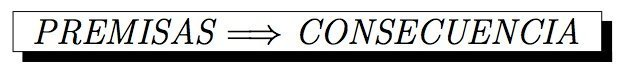
\includegraphics[width=0.6\linewidth]{images/Figura-premisas-consecuencia}\label{fig:figure}
\end{figure}
Entonces, ¿qué es un razonamiento?
Un razonamiento es una cadena de argumentos que llevan desde las premisas a la consecuencia.
El razonamiento es correcto cuando cada argumento es lógicamente correcto.
Por tanto, si el teorema es de la forma
\[
    P \implies Q
\]
donde $P$ es la premisa y $Q$ la consecuencia, la demostración es una cadena de argumentos lógicamente correctos que parte de las premisas y acaba en la conclusión, como la siguiente:
\[
    P \implies R_1 \implies R_2 \implies \ldots \implies R_k \implies Q
\]
donde cada $R_i$ es un razonamiento intermedio.
Un teorema puede ser demostrado con diferentes pruebas (unas serán más elegantes y simples que otras).
Veamos la demostración del teorema 1.
Empezamos por aplicar la definición de divisibilidad a los enteros $a$ y $b$.
\begin{proof}
    Como $a$ divide a $b$, entonces existe un entero $k_1$ tal que $b = a \cdot k_1$.
    Análogamente, como $b$ divide a $c$, existe otro entero $k_2$ tal que $c = b \cdot k_2$.
    \par\textbf{\small(La siguiente idea es combinar las dos igualdades obtenidas.)}\par
    Dado que $b = a \cdot k_1$ y $c = b \cdot k_2$, podemos sustituir $b = a\cdot k_1$ en la segunda igualdad:
    \[
        c = b \cdot k_2 = a\cdot k_1 \cdot k_2 = a\cdot (k_1 \cdot k_2).
    \]
    \textbf{\small(Finalmente, anunciamos la consecuencia del teorema, que es una consecuencia lógica del argumento.)}\par
    La igualdad $c = a \cdot (k_1 \cdot k_2)$ significa que $a$ divide a $c$.
    Por tanto, la propiedad de divisibilidad es transitiva.
\end{proof}
El símbolo \qedsymbol\ se coloca al final de una prueba para indicar su fin.
También se emplea el acrónimo QED, que en latín significa “como queríamos demostrar”.

Hay una cuestión a la que los estudiantes tienen que prestar atención: las definiciones.
Muchos estudiantes escriben demostraciones incorrectas porque no saben o no recuerdan las definiciones.
Las definiciones son términos que fijan el significado de objetos y propiedades matemáticos.
Por ejemplo, se define el valor absoluto porque es una función que aparece con suma frecuencia; en este caso, la definición se ha hecho por concisión y comodidad de uso.
En cambio, la definición de continuidad recoge una propiedad abstracta, el que límite en un punto coincida con el valor de la función.
Los términos matemáticos tienen significado diferente al que poseen en el lenguaje natural.
Antes de escribir una prueba es una buena idea revisar las definiciones pertinentes.
    \section{Tipos de demostración}

Según la naturaleza del teorema o del problema que resolver, es preciso o recomendable un tipo de demostración particular.
En lo que sigue estudiaremos los distintos tipos de demostración y los contextos en que aparecen.

\subsection{Demostración directa}

Una demostración directa es una demostración en que se aplican directamente resultados y definiciones que se dan por conocidos.
La estructura de la demostración consiste en una cadena de implicaciones.
He aquí un ejemplo de este tipo de demostración.

\begin{theorem}
    Sea $n$ un número natural.
    Si al dividir $n$ por 3 da como resto 2, entonces, $n^3 + 1$ es divisible por 3.
\end{theorem}
\begin{proof}
    Si $n$ da 2 como resto al dividirlo por 3, esto significa que existe un entero $q$ tal que $n = 3q + 2$.
    Sustituimos en $n^3 + 1$ y desarrollamos:
    \[
        n^3 + 1 = (3q + 2)^3 + 1 = (27q^3 + 54q^2 + 36q + 8)+ 1 = 3(9q^3 + 18q^2 + 12q + 3)
    \]
    Se sigue que el último número obtenido es un múltiplo de 3 y, por tanto, el teorema es cierto.
\end{proof}

\subsection{Demostración por casos}

A veces la estructura lógica de un teorema es de la forma $(P_1 \land P_2 \land \cdots \land P_k) \implies Q$, esto es, la premisa del teorema se puede descomponer en la disyunción de otras premisas, los casos.
La estructura lógica es equivalente a $(P_1 \implies Q) \land (P_2 \implies Q) \land \ldots \lands (P_k\implies Q)$.
La demostración del teorema consiste en probar por separado que la conclusión Q se sigue de cada caso $P_i,\ i = 1, \cdots,k$.
La prueba del siguiente teorema se ha escrito por casos.
\begin{theorem}
    El producto de dos enteros consecutivos es siempre un número par.
\end{theorem}
\begin{proof}
    Sea $x$ un entero.
    Dividimos en dos casos la prueba, según $x$ sea par o impar.
    \begin{itemize}
        \item El caso en que $x$ es un número par.
        En este caso, $x$ se puede escribir como x = 2k, para cierto entero k.
        Entonces el producto $x(x + 1) = 2k(2k + 1)$, que es un número par.

        \item El caso en que $x$ es un número impar.
        Ahora $x = 2k + 1$, para cierto entero k.
        Se sigue que $x(x + 1) = (2k + 1)(2k + 1 + 1) = (2k + 1)(2k + 2) = 2(2k + 1)(k + 1)$.
        Esto implica que $x(x + 1)$ es par.
    \end{itemize}
\end{proof}



\subsection{Demostración por reducción al absurdo}

Este tipo de pruebas se llama también demostración por contradicción. Se niega la conclusión del teorema y se incorpora como una premisa más. A partir de ahí, se razona lógicamente hasta alcanzar una contradicción con alguna de las premisas del teorema. Como se ha obtenido una contradicción, no es posible la negación de la conclusión, y el teorema es cierto. A continuación se presenta una demostración por reducción al absurdo muy conocida.

Teorema 6 Probar que el conjunto de los números primos es infinito.

Prueba: Supongamos que hubiese un número finito de primos, digamos, {p1,p2,…,pn}. Construimos un nuevo número p como sigue:
p = p1 ⋅p2 ⋅...⋅pn + 1
La pregunta ahora es si p es primo o no. No puede ser compuesto, porque entonces algunos de los primos p1,…,pn tendría que dividir a p. Por su construcción, eso es imposible. Se sigue que p es primo. Esto contradice el hecho de que haya exactamente n primos. QED



3.4 Demostración por contraposición
A veces la demostración directa de un resultado resulta ser bastante difícil o enrevesada. Sin embargo, cuando el resultado se formula por contraposición la prueba se puede tornar fácil. Si el teorema tiene la estructura lógica P= ⇒Q, su contrapositivo es ¬Q= ⇒¬P. El ejemplo siguiente ilustra esta técnica.

Teorema 7 Sea n un número entero. Si n2 es par, entonces n es par también.

Prueba: Supongamos que n no es par. Entonces n se puede escribir como n = 2k + 1, para cierto entero k. Sustituyendo en n2 tenemos:

n2 = (2k + 1)2 = 4k2 + 4k + 1 = 2(2k2 + 2k) + 1
Esto prueba que n2 es impar. Por el contrapositivo, hemos probado que si n2 es par, entonces también lo es n. QED

Aunque algunos alumnos las confunden, la demostración por contraposición es distinta a la demostración por reducción al absurdo. En esta última prueba es necesario obtener una contradicción, pero no así en la demostración por contraposición.


3.5 Demostración por inducción
Las demostraciones por inducción aparecen cuando el enunciado del teorema asevera que una propiedad P(n) es cierta para cualquier n ∈ ℕ, siendo P(n) una propiedad que depende de los números naturales. Consta de dos partes: una, llamada paso base, donde se demuestra que la propiedad es verdadera para un cierto n0; y otra, llamada paso inductivo, donde se prueba que, si P(n- 1) es cierta para n > n0, entonces P(n) es cierta. Si ambos pasos se demuestran correctamente, entonces P(n) es cierta para n ≥ n0. El teorema que viene a continuación presenta una sencilla prueba por inducción.

Teorema 8 Demostrar que para todo número natural n se cumple la fórmula:
n(n-+-1)
1 + 2 + ...+  n =    2
Prueba: La prueba tiene dos pasos, el paso base y el paso inductivo.
Paso base. Se comprueba que la fórmula es cierta para n = 1. El miembro izquierdo de la fórmula da 1; el derecho, 1(1+ 1)
--------
2 = 1, con lo cual la fórmula se cumple.
Paso inductivo. Ahora probaremos que si la fórmula es cierta para n-1, entonces también es cierta para n. La fórmula para n - 1 tiene la siguiente forma (sustitúyase n por n - 1):

(n - 1)n
1+  2+ ...+ (n - 1) = --------
2

Escribimos la suma de los n primeros números y aplicamos la fórmula anterior:


El último término obtenido es la fórmula para n. Luego la fórmula es correcta para cualquier n ∈ ℕ. QED



3.6 Demostración constructivas
Las demostraciones constructivas, a diferencia de por ejemplo las de por reducción al absurdo, construyen explícitamente el objeto matemático que se pide en el enunciado. Se da con frecuencia en la resolución de problemas. En el resultado siguiente se pide construir las soluciones de la ecuación ax2 + bx + c = 0 y se da una demostración constructiva.

Teorema 9 Sean a,b,c tres números reales con a no nulo. Probar que la ecuación ax2+bx+c = 0 tiene siempre solución, bien sea real o imaginaria.

Prueba: Para construir la solución vamos a completar los cuadros en la ecuación. Primero, sacamos factor común a, puesto que a ⁄= 0, y después sumamos y restamos el término b2∕4a2:

A continuación, completamos los cuadrados:

Por último, despejamos la x:

Según el valor de b2 - 4ac, tenemos tres casos: (1) raíces reales simples, cuando b2 - 4ac sea estrictamente positivo; (2) raíz real doble, cuando b2 - 4ac sea nulo; (3) y raíces complejas conjugadas, cuando b2 - 4ac sea estrictamente negativo. QED



    \section{Refutaciones y contraejemplos}

En matemáticas siempre se pregunta qué pasa con el recíproco de una implicación. Se enuncia un teorema que tiene la clásica estructura P=⇒Q y nos preguntamos: “¿Será cierto también que Q=⇒P, su recíproco?” Muy a menudo, ocurre que el recíproco no es cierto. Pero ¿cómo se prueba que una implicación es falsa? Por medio de un contraejemplo. Un contraejemplo es un caso en que las premisas son ciertas, pero la conclusión es falsa. Exhibir un contraejemplo es refutar una implicación. Pongamos como ejemplo el conocido teorema de que toda función derivable en un punto es continua. La demostración consta de una línea; si f(x) es derivable en x = a, entonces:


f(x)---f(a)               f(x)--f(a)-               ′
lxim→a(f(x)- f (a)) = lxim→a    x - a   ⋅(x - a) = lix→ma    x - a    ⋅ lxim→a(x - a) = f(a) ⋅0 = 0
Ahora bien, ¿es cierto el recíproco, que toda función continua es derivable? No, y el contraejemplo lo constituye la función f(x) = ∣x∣ en x = 0. Los siguientes cálculos lo prueban:


(
(                          |       ∣x∣---∣0∣-
|{  xl→im0+ x = 0              ||{  lx→i0m+     x    = 1
(1) lim ∣x∣ =                        (2)
x→0      |(   lim  (- x) = 0           |||       ∣x∣-  ∣0∣
x→0-                    (  lx→i0m- ---x----= - 1
En (1) se demuestra que el valor absoluto es continuo; en (2), que no es derivable, ya que los límites laterales de la derivada son distintos. Esto es un contraejemplo de que las funciones continuas son derivables. Obsérvese que basta dar un solo contraejemplo para invalidar la implicación entera.
Por último, por mor del desafío intelectual, hay autores que presentan problemas que aparentemente contienen algún tipo de trampa. Una vez más, se resuelven a base de imaginación y lógica. A continuación reproducimos un conocido problema de esta categoría (tomado del excelente libro ¡Ajá!, de Martin Gardner [Gar89]).

Problema 10 En su lecho de muerte un beduino reparte la herencia a sus tres hijos. El hombre comunica a sus hijos que les deja 11 camellos que han de repartirse como sigue: 1∕2 de los camellos para el mayor, 1∕4 para el mediano y 1∕6 para el pequeño. Sin embargo, no saben cómo llevar a cabo el reparto, ya que ni 2, ni 4, ni 6 dividen a 11. Piden ayuda a un sabio, quien acude servicial a la casa del beduino en camello. Tras escuchar a los hijos, decide regalarles su camello para facilitar el reparto. Entonces ahora hay 12 camellos. Al mayor le corresponden 6, al mediano 3 y al menor 2. En total, se han repartido 11 camellos. El sabio toma su camello otra vez y vuelve a su casa. ¿Cómo pudo hacer el reparto?


    \section{a}
    \section{Principios generales de escritura}

En esta sección vamos a enunciar unos principios generales para escribir matemáticas, aunque, en realidad, se aplican a muchos otros tipos de escritura. El lector se dará cuenta de que estos principios se basan lisa y llanamente en el sentido común y que todos persiguen el objetivo de hacer de un texto matemático un acto sereno y profundo de comunicación.

\hspace{5mm}\textbf{Claridad.}
Nada se puede comunicar si previamente el autor no tiene una idea clara de ello.
Tan clara tiene que estar la idea en la mente del autor que este tiene que estar ansioso por comunicarla.
Pero la idea tiene que transmitirse de modo inteligible, presentarse en un orden racional, fruto de la reflexión, podando los detalles que resulten innecesarios al lector ideal de nuestro texto.
Por ejemplo, si la demostración va a ser larga, es útil describir al lector el plan general de un modo informal, y luego pasar a los detalles técnicos de modo formal.

\hspace{5mm}\textbf{Concisión.}
La concisión es difícil de alcanzar y lleva mucha práctica.
La concisión es el arte de significar lo más posible con el menor número de palabras.
Un texto conciso está bien cimentado y en él no sobra ni falta nada.
La concisión se alcanza a través de un proceso de depuración del texto que incluye, entre otros, los siguientes procesos:
eliminar palabras con poco significado (redundancias, palabras que no maticen, muletillas);
descartar el material que el lector pueda deducir por sí mismo;
cuando sea posible, sustituir subordinadas adjetivas por adjetivos;
usar palabras precisas y cortas en lugar de perífrasis;
eliminar temas secundarios que afecten al tema principal (más tarde se pueden comentar, pero una vez dicho lo esencial).

\hspace{5mm}\textbf{Simplicidad.}
Relacionadas con los dos puntos anteriores está la simplicidad.
No debe confundirse simplicidad con pobreza de escritura.
La primera se refiere a una organización de la escritura que es inmediatamente inteligible y transparente;
la segunda, precisamente, a una falta de ello por defecto.
La simplicidad es una cuestión de estilo matemático también.
Un teorema se puede probar por más de un camino y a veces el camino más corto es el preferible.

\hspace{5mm}\textbf{Escritura en frases y párrafos.}
Este punto puede parecer totalmente superfluo, por obvio, pero la experiencia demuestra que no se insiste lo suficiente. En un texto matemático, como en cualquier otro, las ideas deben organizarse en frases, con su sentido completo, y estas, a su vez, en párrafos. Cada párrafo debe contener una idea principal, la cual se explica en frases claras y concisas. Mezclar ideas distintas en un mismo párrafo es una mala práctica y habla penosamente de la claridad mental del autor sobre el tema en cuestión. Una cuestión importante es la puntuación, que cuando se utiliza de modo cabal, ayuda enormemente a estructurar el texto y dotarlo de claridad en sus partes.

\hspace{5mm}\textbf{Precisión.}
En matemáticas el lenguaje es extremadamente preciso. Usarlo sin esa precisión conduce a sumir al lector en una profunda confusión. Por ejemplo, hay diferencias entre expresión, igualdad, ecuación y fórmula, y cuando se escribe hay que tenerlas en cuenta. Una expresión es una sucesión de símbolos que expresa una relación matemática; por ejemplo, x2 + 2x + 1 es una expresión. Una igualdad establece que dos expresiones son iguales y siempre lleva el signo “=”; por ejemplo, (3x- 1)2 = 8x2 - 4x es una igualdad. Si la igualdad tiene carácter cuantitativo, se habla de ecuación y está se puede resolver; en el ejemplo anterior, la única solución es x = 1. Una fórmula es una igualdad que tiene carácter general; se habla de la fórmula del área del círculo A = πr2, pero no de la igualdad entre A y πr2.

\hspace{5mm}\textbf{Uso juicioso de los símbolos matemáticos.}
Un texto matemático sigue siendo un texto y no hay que sustituir las palabras por símbolos, pues lo hace intricado de leer. Debería resistirse el uso de los símbolos tanto como sea posible. Expliquemos las matemáticas con palabras del castellano mientras la necesidad de formalización no nos obligue a usar símbolos. No hay cosa más farragosa de leer que un texto matemático en que se han sustituido un gran número de palabras por símbolos matemáticos. Es preferible escribir para todo número real que ∀x ∈ ℝ. Todo símbolo matemático ha de tener necesariamente una función gramatical dentro de la frase.

Algunos símbolos pueden actuar como verbos; por ejemplo, x = y es equivalente a x es igual a y. Pero la expresión x2 + 2x + 1 no tiene verbo y ha de tratarse como un nombre; por ejemplo, x2 + 2x + 1 es siempre positiva para todo x. Cuando los cálculos son largos conviene ponerlos en una línea aparte y centrados:

Si es necesario, se pueden dividir un cálculo largo en varios cálculos más pequeños y explicar cada uno con palabras.

\hspace{5mm}\textbf{Organización del texto.}
Como cualquier otro texto de envergadura, un texto matemático necesita planificación. Antes de escribirlo, tenemos que tomar notas, visualizar mínimamente sus partes y cuál va a ser su orden, imaginar el nivel de conocimiento de nuestro lector, en qué conceptos vamos a hacer más énfasis, cuál va a ser el nivel de repetición, entre otros. Ponerse a escribir sin haber planificado el texto es lo que se llama escribir por acumulación. Vamos sumando párrafo tras párrafo, trabajosamente, con penuria, pero nada tiene coherencia ni estructura y faltan detalles esenciales, pues el autor no previó nada. El lector se percata de esto tras la lectura de las primeras frases y ya alberga sospechas inquietantes de las intenciones del autor y el texto.

\hspace{5mm}\textbf{Aspectos formales del texto.}
Hay que cuidar el contenido matemático y la corrección lingüística. Si falla cualquiera de estos dos elementos, el texto se vuelve insufrible. Sobre la corrección lingüística, se profundizará en la sección 7. Respecto al contenido matemático, aquí ofrecemos unos mínimos consejos de sentido común: (1) como hemos dicho, hay que cuidar el uso de los símbolos, su encaje en las frases, y, a ser posible, emplear el número exacto de símbolos; (2) asimismo, hay que numerar claramente los resultados para que sea fácil referirse a ellos más tarde; (3) hay que ser consistente con la notación y usar la que está aceptada por convención; (4) usar figuras para ilustrar demostraciones; (5) dar formato al documento de manera que sea cómodo de leer.

\hspace{5mm}\textbf{Revisión continua del texto.}
Una clave para escribir un buen texto es la revisión, y con esto queremos decir la revisión continua del texto. Como consecuencia de esas revisiones, volveremos a escribir y a escribir párrafos enteros. No pasa nada. Si el resultado final es un texto bien escrito, todas esas revisiones merecen la pena. Algunas revisiones tienen que tener un criterio específico. Por ejemplo, una serie de revisiones deberían ser gramaticales; otra, del contenido matemático; otra, de la estructura en párrafos; otra, del ritmo y la fluidez del texto; otra, del léxico y las repeticiones sintácticas; otra del orden de las partes. Además, mi consejo es que, tras trabajar en el texto intensamente durante unos días, nos olvidemos de él, y tras un cierto tiempo volvamos a revisarlo de nuevo con renovada exhaustividad. Tras ese paréntesis se borra la huella mental, que en ocasiones nos hace pasar por alto errores y aceptar como bueno lo escrito (cuando, probablemente, no lo es). La lectura de nuestro documento debe hacerse con mucha atención y despacio; no es una lectura rápida en absoluto. Algunos autores recomiendan leer en voz alto para forzar la lectura lenta y comprensiva (véase Kevin Houston [Hou13]). El matemático Paul Halmos en su famoso ensayo How to write mathematics [Hal70] recomienda escribir en espiral. Si un texto va a tener, digamos, 5 párrafos, una posible sucesión de escritura podría ser 1 - 2 - 1 - 2 - 3 - 1 - 2 - 3 - 4 - 1 - 2 - 3 - 4 - 5. En realidad, el método que predica Halmos combina escritura y revisión en el mismo proceso.
    \section{El castellano es un bello idioma}

Un texto matemático sigue siendo un texto escrito en una lengua, en este caso el castellano, que cuenta con sus normas ortográficas, gramaticales, léxicas y discursivas.
Es menester respetarlas, no desde la coerción, sino desde la naturalidad e incluso el disfrute.
Ante este tema, lamentablemente, de nuevo nos encontramos con una situación incómoda y triste.
Para su vergüenza, muchos profesores de ciencias piensan que ``escribir bien es cosa de la gente de letras''.
No es cierto.
Escribir bien es cosa de gente con cultura y claridad de pensamiento; en particular, es un asunto de relevancia para cualquier profesor de universidad que se precie de serlo.
Para su vergüenza, un nutrido grupo de alumnos piensa igual, unos animados por lo que oyen a esos profesores, otros conscientes de que escribir no impide aprobar exámenes, sacar buenas notas en trabajos escritos, y aún menos sacar un título universitario.
Anteriormente hemos ofrecido argumentos contundentes (sección 1) para rebatir la perniciosa idea de que en las clases de ciencias no hay que saber escribir bien.
No insistiremos más en ellos. En esta sección vamos entrar en los detalles de la corrección lingüística, asunto espinoso con el que pocos profesores de ciencias se atreven a tratar.
Nuestros textos tienen que estar escritos en un castellano correcto y, si ello es posible, con voluntad de estilo.
Hemos dividido los errores en las siguientes categorías: ortográficos, gramaticales y léxicos.
Obviamente, no vamos a cubrir extensamente cada una de las categorías, sino que haremos énfasis en los errores más frecuentes que se encuentran en la escritura de textos matemáticos.


\subsection{Errores ortográficos}

Quizás uno de los errores más frecuentes es la acentuación incorrecta (¿o deberíamos decir la falta de acentuación?).
La tilde, ese símbolo ortográfico que usamos para identificar la sílaba tónica, tiene también la función de distinguir palabras.
Así, no es lo mismo escribir perdida y referirse a una ocasión que a la muerte de un ser querido, en cuyo caso sería pérdida.
Una acentuación incorrecta distrae al lector, pues le fuerza a pararse y averiguar a cuál de los posibles significados se está refiriendo el autor.
Ello causa una irritación soterrada y predispone al lector contra el texto.
¿Cómo puede confiar un lector exigente, tal como un profesor de universidad, en que el texto es tiene calidad si la acentuación es confusa y errática?

Ante nuestras quejas por la acentuación incorrecta, algunos alumnos nos han contestado, a veces de modo desafiante, que lo habían pasado por el corrector de Word.
Si hay dos palabras que se escriben exactamente igual salvo por el acento el corrector de Word no detectará la diferencia, pues no es capaz, de momento, de discriminar en función de la semántica (del significado).
Recomendamos al lector que repase las reglas de acentuación y use su capacidad mental en lugar de confiar ciegamente en el Word; además, este no les valdría en un examen, por ejemplo.
Para un repaso de las reglas de acentuación, véase el artículo sobre la tilde del Diccionario panhispánico de dudas [RAE13a] (DPD a partir de ahora).
Y, sí, el examen es de inglés.

Otro punto donde se observan numerosos casos de incorrección es en el uso de las mayúsculas.
Quizás sea por la influencia de inglés, pero nos encontramos con usos que corresponden a sus reglas en lugar de a las del castellano.
Los días de la semana, los meses del año y las estaciones se escriben en minúscula: lunes, junio y otoño, y no $\bigotimes$Lunes, $\bigotimes$Junio y $\bigotimes$Otoño (usamos el símbolo $\bigotimes$ para indicar ejemplos de incorrecciones).
Otros errores relacionados con el uso de las mayúsculas en los textos matemáticos son los siguientes:
\begin{enumerate}
    \item Los nombres de los teoremas van en minúsculas: teorema fundamental del cálculo y no $\bigotimes$Teorema Fundamental del Cálculo.
    \item Los nombres de las disciplinas científicas en el contexto académico (asignaturas, grados, materias de estudio) van en mayúsculas: Soy licenciado en Informática.
    En caso contrario, van en minúscula: Ninguna persona puede abarcar las matemáticas actuales.
    \item Los títulos de los trabajos no llevan la mayúscula inicial de cada palabra.
    Esa es una norma inglesa.
    Es incorrecto escribir en el título de un trabajo $\bigotimes$El Método de la Bisección.
\end{enumerate}


Para más información, véase el artículo sobre el uso de las mayúsculas en el DPD [RAE13c].
Y por último, entramos en uno de los grandes problemas de nuestros alumnos y que más confusión causan: la puntuación. Un texto mal puntuado rompe constantemente las expectativas de lectura y se convierte pronto en un galimatías. La puntuación está pensada para cimentar la estructura del texto, para matizar sus distintas partes, para guiar en la lectura fluida del texto. Cuando se usa contra natura consigue los efectos más perversos; el más inmediato, la sensación de chapuza. Un texto mal puntuado habla elocuentemente de la confusión de ideas y de la falta de capacidad para revisar un escrito de su autor.


Vamos a repasar brevemente los principales usos de la puntuación; de nuevo, se remite al lector a los excelentes artículos del DPD [RAE13b, RAE13d]

\textbf{Uso de la coma.}\par
Quizás el signo de puntuación más potente y al mismo tiempo más difícil de usar.
La coma sirve principalmente para separar partes de la oración. El uso de la coma es obligatorio en ciertos casos (el llamado uso normativo) y en otros es la elección del autor (uso estilístico). La coma se usa en los siguientes casos:


En las aposiciones explicativas (interrupciones hechas en la oración para explicar algo): La función f(x), que es continua y derivable, tiene un único máximo en [0,1].
Coma de enumeración: Se pone cuando se hace una enumeración de objetos. Si los dos últimos elementos van unidos por la conjunción y u o, no hay coma entre ellos: La función tiene máximos relativos en x = 1, x = 3
2 y x = 5.
Coma elíptica. Cuando se repite el verbo en dos oraciones seguidas, la segunda vez se puede sustituir por una coma: La función f(x) es continua; su derivada, no. En este caso es recomendable usar el punto y coma tal cual aparece en el ejemplo anterior.

Coma delante de las conjunciones. Se pone coma delante de las conjunciones (o locuciones conjuntivas) que unen dos oraciones compuestas. Ejemplos de esas conjunciones son: pero, aunque, sino que (adversativas); así que, de manera que, conque, luego (consecutivas o ilativas); esto es, o sea, es decir (explicativas). Por ejemplo: La sucesión an es creciente, pero ello no implica que tienda a infinito. En el caso de las oraciones causales la coma se coloca según su tipo. Las oraciones causales se clasifican en causales lógicas, en que una oración se deduce de la otra, y las causales enunciativas, en que se enuncia algo como consecuencia lógica de otro hecho. Por ejemplo, n2 es par, porque n es par es causal lógica y n es par porque n2 es par es causal enunciativa. En las causales lógicas se separan las oraciones por una coma y en las causales enunciativas, no.

Coma sintáctica. En ocasiones, por propósito de énfasis o estilo, se invierte el orden natural de las partes de la oración. En este caso, ello se advierte poniendo una coma detrás de la parte anticipada, sobre todo si esa parte es muy larga. Se separa con coma en En el conjunto de los números enteros y bajo ciertas condiciones, es posible extender la función f(x), pero no en Elegante es esta demostración. Este es uno de los casos donde la coma tiene un uso opcional, pero que siempre debería estar sancionado por el sentido común. Es obligatorio poner la coma en el caso de las oraciones adverbiales, cuando la subordinada está antepuesta: Antes de que pasemos a estudiar la continuidad, vamos a calcular el dominio de la función.

Coma para evitar la ambigüedad. Este uso no es normativo, pero una lectura atenta del texto indica enseguida dónde ponerlo. No es lo mismo Me vestí, como me indicaron (me vestí porque me invitaron a ello) que Me vestí como me indicaron (me vestí en la forma en que me indicaron). Y, no, no somos caníbales.

Usos fijos. Se pone coma después de ciertos enlaces, tales como en primer lugar, por lo tanto, por otro lado, por último, con todo, sin embargo, no obstante, y también después de locuciones adverbiales cuando afectan a la frase entera: Por lo tanto, las funciones derivables son continuas.

Separación de sujeto y verbo. Salvo que medie una aposición explicativa, no se usa coma para separar el sujeto y el verbo: ○xToda sucesión creciente y acotada, tiene límite.


Uso del punto y coma. Por alguna razón misteriosa los estudiantes usan poco este signo de puntuación. Es un error, ya que es tremendamente versátil a la hora de organizar un texto y separar con claridad sus partes.
Enumeraciones complejas.Se usa en este caso cuando la enumeración es larga o los elementos de la enumeración llevan comas también: La integral consta de: los límites de integración, escritos abajo y arriba del símbolo ∫ ; el integrando, escrito a continuación; y el diferencial dx, que indica respecto a qué variable se integra.
Separación de oraciones. En castellano la manera de separar oraciones sintácticamente independientes pero con relación semántica es con punto y coma, y no con coma. Por ejemplo: Vemos que, para K arbitrario, existe un n0 tal que an > K si n > n0; no se puede concluir que el límite de an exista.
Para separar conectores. Siguiendo con el punto de más arriba sobre usos fijos de la coma, con conectores de sentido adversativo, consecutivo o concesivo se pone una coma tras ellos, sobre todo cuando se unen dos oraciones en una más larga: Si la serie converge, entonces su término general tiende a cero; no obstante, el recíproco es falso.
Enumeraciones en varias líneas. En una lista que se escribe en líneas independientes se pone punto y coma en cada línea, salvo en la última que se pone punto:
Sea G un grafo. Las siguientes condiciones son equivalentes:

el grafo G es conexo;

existe un camino entre dos vértices arbitrarios del grafo;

no existen aristas puente en el grafo.


\subsection{Errores gramaticales}
Los errores más comunes que nos hemos encontrado en los trabajos escritos de los alumnos son los siguientes:

Errores de sintaxis. El orden de las partes de una oración es esencial para entender su significado. La elección de ese orden ha de estar guiado por un afán de máxima claridad. Por ejemplo, la frase ○xVamos a calcular la derivada de la función segunda es incorrecta; el lector no sabe si se refiere a la segunda de dos funciones o a la derivada segunda de una única función. Debería haberse escrito Vamos a calcular la derivada segunda de la función.
Errores de concordancia. En general, estos errores aparecen por una falta de revisión del texto. El estudiante cambia una parte de la frase y no tiene el rigor metodológico de revisar cómo afecta ese cambio al resto de la oración. Un caso que sí es frecuente es el del uso impersonal del verbo haber. Este verbo, cuando se usa como impersonal, no tiene sujeto y se conjuga en la tercera persona del singular: hay, ha habido, hubo, etc. Así, es incorrecto decir ○xHan habido dos soluciones de la ecuación, y lo correcto es Ha habido dos soluciones de la ecuación.
Errores en los verbos. Cuando el alumno no tiene clara una demostración o la solución de un problema, a veces tiende a disfrazarlo mediante el uso incorrecto de las perífrasis verbales. Los principales errores se pueden clasificar en tres grupos:

Uso innecesario: x○Hemos sido capaces de demostrar el resultado, que debería decirse simple y llanamente Hemos demostrado el resultado.
Error de construcción, en particular con los complementos de régimen verbal. Estos complementos son los sintagmas preposicionales que van unidos a un verbo y sin el cual este no tiene significado completo; por ejemplo, contar con alguien. Es incorrecto decir x○El resultado depende el teorema 1, sino El resultado depende del teorema 1.
Errores de uso. Uno de los casos más frecuentes es la confusión entre deber y deber de. El primero tiene valor de obligación y el segundo de probabilidad. No se puede decir x○El resultado debe de ser cierto (esto es, el resultado es probablemente cierto), sino El resultado debe ser cierto (esto es, el resultado es cierto con seguridad).


\subsection{Errores léxicos}
Los errores léxicos que hemos observado en nuestros alumnos principalmente se reducen a una sola clase: pobreza léxica. Un texto brilla si se usan diferentes palabras, aunque sea para expresar la misma idea. Cada palabra tiene su matiz, su personalidad, su sonoridad, y una elección cuidada de las palabras dice mucho del texto y, por ende, del autor. La pobreza léxica se caracteriza por el uso de un conjunto pequeño de vocablos para expresar ideas para las cuales existen palabras con más riqueza semántica. Típicamente, en un trabajo escrito un alumno usaría el verbo decir repetidamente, que es un verbo de carácter general; sin embargo, hay otros muchos verbos que expresan matices distintos, tales como comentar, explicar, referir, señalar, glosar, enumerar, argumentar, objetar, replicar, comunicar, entre otros.
    \section{Código interno y otras demostraciones mejorables}


En esta sección analizaremos un par de demostraciones escritas por alumnos (son totalmente reales). Señalaremos cómo mejorarlas aplicando todo lo desarrollado en este documento hasta ahora, tanto de forma como de contenido.

Teorema 12 Demostrar que hay un número infinito de primos.
Prueba: Usando el método de reducción al absurdo, es decir, supondremos que hay un número primo, que llamaremos p, que es el último número primo, esto implicaría que habría un número finito de primos y veremos que esto es imposible.
Suponiendo que p es el número primo más grande y construimos otro número q: q = (2 ⋅ 3 ⋅ 5 ⋅ 7 ⋅… ⋅ p) + 1 que es el resultado de multiplicar todos los números primos hasta el último p; después sumarle 1.
Evidentemente q no es divisible por ningún primo pues siempre daría como resto 1 luego q es divisible solo por 1 y por sí mismo, es decir, q es primo. Por otra parte q es mayor que p. Luego p no es el mayor número primo. Por tanto no puede existir un número primo que sea el mayor y con esto verificamos la existencia de infinitos números primos.

Analizaremos párrafo por párrafo. Empezamos con el primero:
Usando el método de reducción al absurdo, es decir, supondremos que hay un número primo, que llamaremos p, que es el último número primo, esto implicaría que habría un número finito de primos y veremos que esto es imposible.

El párrafo tiene que dividirse en frases. Las frases se amontonan unas tras otras separadas por comas; faltan conectores que las unan con sentido.
Se mezclan los tiempos verbales (supondremos, llamaremos, implicaría, veremos).
Es incorrecto gramaticalmente empezar con un gerundio y luego continuar con el futuro.
El párrafo no es conciso porque no es claro. Es breve, pero confuso.
La muletilla es decir sobra. También se puede decir por reducción al absurdo en lugar de método de reducción al absurdo; aquí método no aporta nada.
El autor informa al lector del plan de la prueba y esto está bien.
Para el segundo párrafo:
Suponiendo que p es el número primo más grande y construimos otro número q: q = (2 ⋅ 3 ⋅ 5 ⋅ 7 ⋅… ⋅ p) + 1 que es el resultado de multiplicar todos los números primos hasta el último p; después sumarle 1.

La conjunción y en la frase Suponiendo que p es el número primo más grande y construimos otro número q es incorrecta; distrae de la lectura.
Lo normal habría sido poner la fórmula q = (2 ⋅ 3 ⋅ 5 ⋅ 7 ⋅… ⋅ p) + 1 en una línea aparte y centrada.
El párrafo está mal puntuado; en particular, después de la fórmula para q.
La última frase después sumarle 1 está incompleta, le falta el verbo. No es una explicación clara para el lector, sino una suerte de orden.
Para el último párrafo:
Evidentemente q no es divisible por ningún primo pues siempre daría como resto 1 luego q es divisible solo por 1 y por sí mismo, es decir, q es primo. Por otra parte q es mayor que p. Luego p no es el mayor número primo. Por tanto no puede existir un número primo que sea el mayor y con esto verificamos la existencia de infinitos números primos.

El párrafo está faltamente puntuado. Véase la explicación sobre las oraciones causales y su puntuación en la sección anterior. Las expresiones evidentemente, pues, luego, por otra parte, por tanto llevan coma. Véase la corrección más abajo.
No hemos verificado que la existencia de infinitos números primos (no los hemos contado), hemos demostrado que hay infinitos. Hay que ser precisos con el lenguaje.
He aquí una posible reescritura de la prueba de este alumno; hemos seguido en lo posible el espíritu de su prueba (compárese con la prueba dada anteriormente).

Teorema 13 Demostrar que hay un número infinito de primos.
Prueba (corregida): Probaremos el resultado por reducción al absurdo. Supondremos que hay un número primo, al que llamaremos p, que será el primo más grande. Esto implica que hay un número finito de primos. Veremos que esto es imposible.

Construimos otro número q como sigue:
q = 2 ⋅3⋅5 ⋅7⋅...⋅p + 1
Evidentemente, q no es divisible por ningún primo entre 2 y p, pues su división siempre daría como resto 1. En consecuencia, q es divisible solo por 1 y por sí mismo, es decir,q es primo. Por otra parte, q es un primo mayor que p. Por tanto, p no es el mayor número primo, como habíamos supuesto antes, y esto es una contradicción. Esto prueba que existe un número infinito de primos.

He aquí la segunda prueba:

Teorema 14 Sea p un número primo y a,b números enteros. Probar que si p∣(a ⋅ b), entonces es cierto que o bien p∣a o bien p∣b.
Prueba: Suponemos que p ⁄∣b lo que implica que máximo común divisor entre ellos es 1, de este modo, existe un x1 y x2 que: px1 + ax2 = 1, multiplicamos los dos términos por b, quedando pbx1 + abx2 = b; como p∣a ⋅ b, obtenemos que ab = kp, siendo k un entero, sustituyendo, pbx1 + kpx2 = b, sacamos factor comun p=⇒p(bx1 + kx2) = b, con esto comprobamos que efectivamente p, si divide al menos a uno de ellos, p∣b.

Como vemos la prueba solo consta de un párrafo.
Suponemos que p ⁄ ∣b lo que implica que máximo común divisor entre ellos es 1, de este modo, existe un x1 y x2 que: px1 + ax2 = 1, multiplicamos los dos términos por b, quedando pbx1 + abx2 = b; como p∣a ⋅ b, obtenemos que ab = kp, siendo k un entero, sustituyendo, pbx1 + kpx2 = b, sacamos factor comun p=⇒p(bx1 + kx2) = b, con esto comprobamos que efectivamente p, si divide al menos a uno de ellos, p∣b.

El autor tiene que introducir el siguiente argumento al principio de su prueba o no se comprenderá: Si se tiene que p∣a, entonces la conclusión es cierta. Supongamos entonces que
p ⁄∣b.
Falta una mención explícita al resultado que permite al autor concluir la existencia de x1 y x2, y ese resultado es el teorema de Bezout.
La puntuación del párrafo es nefasta. Además, acumula las frases una tras otra, sin relación entre ellas, separadas por comas que confunden más que ayudan.
El uso del gerundio es incorrecto. Confiere a la prueba una prisa absurda y confirma que el autor escribe por acumulación. Aquí no hay ninguna planificación de la escritura.
En un texto no se puede poner el símbolo =⇒ como sustituto de una implicación. Las palabras priman sobre los símbolos.
El texto parece más el registro de una conversación informal sobre el resultado que un texto matemático propiamente dicho.
He aquí una posible corrección a esa prueba

Teorema 15 Sea p un número primo y a,b números enteros. Probar que si p∣(a ⋅ b), entonces es cierto que o bien p∣a o bien p∣b.
Prueba (corregida): Si se tiene que p∣a, entonces la conclusión es cierta. Supongamos entonces que p ⁄∣b. Esto implica que el máximo común divisor dep yb es 1. Por el teorema de Bezout, existen dos enteros x1 y x2 tal que px1 + ax2 = 1. Si en esta igualdad multiplicamos los dos términos por b, se obtiene pbx1 + abx2 = b. Por hipótesis, sabemos que p∣(a ⋅ b). Esto significa que existe un enterok con ab = kp. Si sustituimos esto en la ecuación antes obtenida tenemos pbx1 + (pk)x2 = b, o lo que es igual, p(bx1 + kx2) = b. De aquí se deduce claramente que p divide a b
    %\section{a}
\end{document}